\subsection{ARM TrustZone}

ARM's TrustZone~\cite{alves2004trustzone} is a collection of hardware modules
that can be used to conceptually partition a system's resources between a
\textit{secure world}, which hosts a secure container, and a \textit{normal
world}, which runs an untrusted software stack. The TrustZone
documentation~\cite{arm2009trustzone} describes semiconductor intellectual
property cores (IP blocks) and ways in which they can be combined to achieve
certain security properties, reflecting the fact that ARM is an IP core
provider, not a chip manufacturer. Therefore, the mere presence of TrustZone IP
blocks in a system is not sufficient to determine whether the system is secure
under a specific threat model. Figure~\ref{fig:trustzone} illustrates a design
for a smartphone \textit{System-on-Chip} (SoC) design that uses TrustZone IP
blocks.

\begin{figure}[hbt]
  \centering
  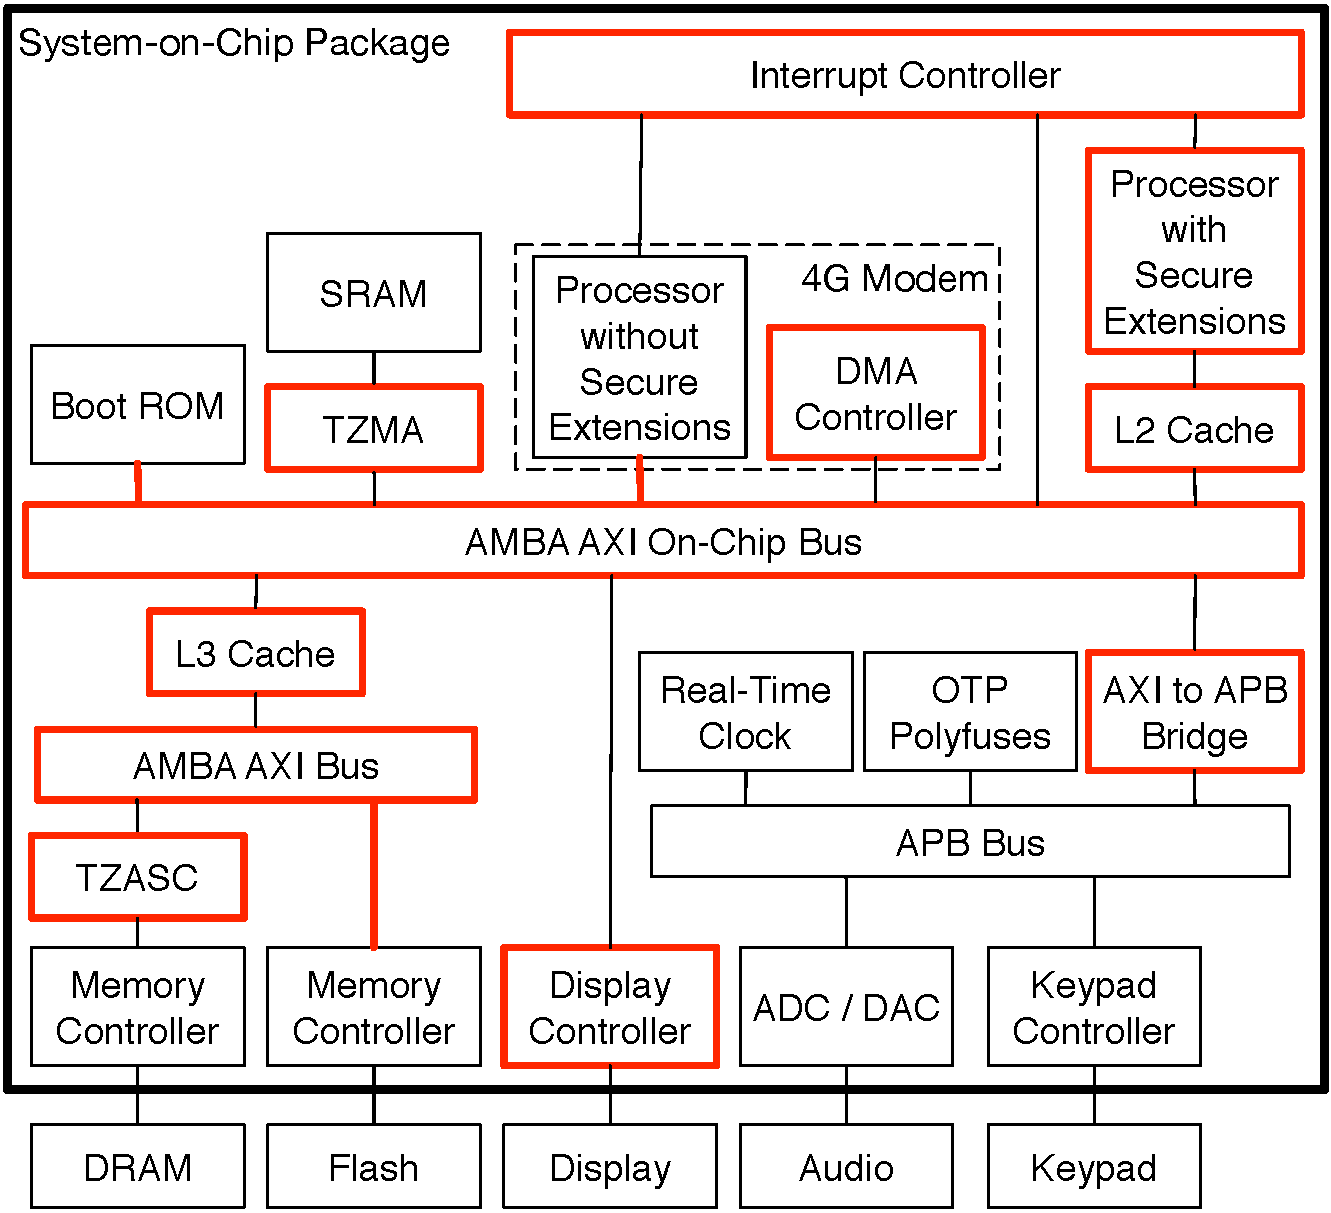
\includegraphics[width=85mm]{figures/trustzone.pdf}
  \caption{
    Smartphone SoC design based on TrustZone. The red IP blocks are
    TrustZone-aware. The red connections ignore the TrustZone secure bit in the
    bus address. Defining the system's security properties requires a complete
    understanding of all the red elements in this figure.
  }
  \label{fig:trustzone}
\end{figure}

TrustZone extends the address lines in the AMBA AXI system
bus~\cite{arm2004ambaxi} with one signal that indicates whether an access
belongs to the secure or normal (non-secure) world. ARM processor cores that
include TrustZone's ``Security Extensions'' can switch between executing code
in the normal world and code in the secure world. The address in each bus
access executed by a core reflects the world that the core is currently
executing in.

The reset circuitry in a TrustZone processor places it in secure mode, and
points it to the first-stage bootloader stored in on-chip ROM. TrustZone's TCB
includes this bootloader, which initializes the platform, sets up the TrustZone
hardware to protect the secure container from untrusted software, and loads the
normal world's bootloader. The secure container must also implement a monitor
that performs the context switches needed to transition an execution core
between the two worlds. The monitor must also handle hardware exceptions, such
as interrupts, and route them to the appropriate world.

The TrustZone design gives the secure world's monitor unrestricted acces to the
normal world, so the monitor can implement inter-process communication (IPC)
between the software in the two worlds. Specifically, the monitor can issue
bus accesses using both secure and non-secure addresses. In general, the secure
world's software can compromise any level in the normal world's software stack.
For example, the secure container's software can jump into arbitrary locations
in the normal world by flipping a bit in a register. The untrusted software in
the normal world can only access the secure world via an instruction that jumps
into a well-defined location inside the monitor.

Conceptually, each TrustZone CPU core provides separate address translation
units for the secure and normal worlds. This is implemented by two page table
base registers, and by having the page walker use the page table base
corresponding to the core's current world. The physical addresses in the page
table entries are extended to include the values of the secure bit to be issued
on the AXI bus. The secure world is protected from untrusted software by having
the CPU core force the secure bit in the address translation result to zero for
normal world address translations. As the secure container manages its own page
tables, its memory accesses cannot be directly observed by the untrusted OS's
page fault handler.

TrustZone-aware hardware modules, such as caches, are trusted to use the secure
address bit in each bus access to enforce the isolation between worlds. For
example, TrustZone's caches store the secure bit in the address tag for each
cache line, which effectively provides completely different views of the memory
space to the software running in different worlds. This design assumes that
memory space is partitioned between the two worlds, so no aliasing can occur.

The hardware modules that do not consume TrustZone's address bit are expected
to be connected to the AXI bus via IP cores that implement simple
partitioning techniques. For example, the TrustZone Memory Adapter (TZMA) can
be used to partition an on-chip ROM or SRAM into a secure region and a normal
region, and the TrustZone Address Space Controller (TZASC) partitions the
memory space provided by a DRAM controller into secure and normal regions. A
TrustZone-aware DMA controller rejects DMA transfers from the normal world that
reference secure world addresses.

It follows that analyzing the security properties of a TrustZone system
requires a precise understanding of the behavior and configuration of all the
hardware modules that are attached to the AXI bus. For example, the caches
described in TrustZone's documentation do not enforce a complete separation
between worlds, as they allow a world's memory accesses to evict the other
world's cache lines. This exposes the secure container software to cache timing
attacks from the untrusted software in the normal world. Unfortunately,
hardware manufacturers that license the TrustZone IP cores are reluctant to
disclose all the details of their designs, making it impossible for security
researchers to reason about TrustZone-based hardware.

The TrustZone components do not have any counter-measures for physical attacks.
However, a system that follows the recommendations in the TrustZone
documentation will not be exposed to physical attacks, under a threat model
that trusts the processor chip package. The AXI bus is designed to connect
components in a SoC design, so it cannot be tapped by an attacker. The
TrustZone documentation recommends having all the code and data in the secure
world stored in on-chip SRAM, which is not subjected to physical attacks.
However, this approach places significant limits on the secure container's
functionality, because on-chip SRAM is many orders of magnitude more expensive
than a DRAM chip of the same capacity.

TrustZone's documentation does not describe any software attestation
implementation. However, it does outline a method for implementing secure boot,
which comes down to having the first-stage bootloader verify a signature in the
second-stage bootloader against a public key whose cryptographic hash is burned
into on-chip \textit{One-Time Programmable} (OTP) polysilicon fuses. A hardware
measurement root can be built on top of the same components, by storing a
per-chip attestation key in the polyfuses, and having the first-stage
bootloader measure the second-stage bootloader and store its hash in an on-chip
SRAM region allocated to the secure world. The polyfuses would be gated by a
TZMA IP block that only makes them accessible to the secure world.
